%To compile, run the following command:
%   latexmk -pdf latex_template.tex 
%
% To edit, you can use your favorite text editor or LaTeX editors such as:
%   Texmaker and TeXworks.
%
% To set up your own TeX system, you can install TeX Live. See:
% https://www.tug.org/texlive/


% For a recent install of texlive on Ubuntu 18.04 that is adequate for
% compiling this file, I used the following commands:
%
% sudo apt install texlive-latex-base
% sudo apt install texlive-latex-extra
% sudo apt install texlive-science

\documentclass[letterpaper,12pt]{article}

\usepackage[margin=1in]{geometry}
\usepackage{amsmath,amsthm,amsfonts,amssymb}
\usepackage{mathtools}
\usepackage{algorithm,algpseudocode}
\usepackage{algorithm}
\usepackage{algpseudocode}
\usepackage{hyperref}
\usepackage{graphicx}
\usepackage{array}
\usepackage{subcaption}

\theoremstyle{remark}
\newtheorem{claim}{Claim}

\DeclarePairedDelimiter\abs{\lvert}{\rvert}
\DeclarePairedDelimiter\floor{\lfloor}{\rfloor}
\DeclarePairedDelimiter\ceiling{\lceil}{\rceil}

\begin{document}

\title{Lab 3: BST Comparison: \\
\large 
Performance analysis and detailed approach
   }


\date{\today}
\author{Qiying Wu}
\maketitle





\section*{Abstract }

 In this lab, we explore the concurrent computation of binary search tree (BST) hashes and tree comparison using Go's concurrency tools, specifically goroutines, channels, and synchronization primitives. The goal is to optimize the processes of hashing, identifying duplicate hash groups, and performing pairwise tree comparisons to achieve high efficiency while maintaining accuracy. Each BST is represented by a unique hash generated from an in-order traversal using a custom hashing function. Multiple configurations of worker threads handle hash computation and map updates, providing insights into the impact of parallelism on performance. This report evaluates the scalability of different parallelization approaches across several worker configurations, with a focus on balancing computational and synchronization overhead.
 
\section*{Introduction }
Binary Search Trees (BSTs) are a fundamental data structure in computer science, used extensively in applications requiring efficient data retrieval and organization. This lab focuses on implementing a parallelized approach to compare BSTs using a custom hash-based methodology. Given a set of BSTs, we aim to compute a unique hash for each tree using an in-order traversal, group trees with identical hashes, and further compare these groups to identify structurally identical trees. Leveraging Go’s concurrency model, the implementation employs goroutines and channels for inter-process communication and synchronization mechanisms such as mutexes and semaphores to ensure data consistency during concurrent hash computations and updates.

The lab is structured in three parts:
\begin{itemize}
 \item \textbf{Hash Computation}: We compute the hash of each BST in parallel by spawning a designated number of worker goroutines, based on the -hash-workers flag. This step evaluates the efficiency of parallel hash computation and measures the time taken to generate hashes for all BSTs.

 \item \textbf{Hash Grouping}: Trees with identical hashes are grouped to identify potential duplicates. Different configurations of data worker goroutines are managed by the -data-workers flag to control access to the map holding hash groups. This part evaluates synchronization overhead and seeks to balance hash computation with data aggregation.

 \item \textbf{Tree Comparison}: For each group with duplicate hashes, tree comparisons are performed in parallel using -comp-workers. This step refines the grouping by identifying structurally identical trees, based on a pairwise comparison strategy.

The experimental setup uses multiple input files with varying BST complexities to analyze the performance of each concurrent approach. The results are assessed for both correctness and performance under different configurations, providing insights into how concurrency levels and synchronization impact the speed and scalability of BST hashing and comparison.
\end{itemize}

This report presents the design and implementation of these different approaches, along with performance analyses based on their execution times for various datasets. We also discuss the challenges encountered during the optimization process, including memory management and non-deterministic behavior caused by atomic operations in CUDA. By comparing the performance of these implementations, we aim to highlight the trade-offs between different levels of abstraction in GPU programming and the impact of hardware-level optimizations on the performance of parallel algorithms like KMeans.



\section{Background and Hashing Methodology}
\subsection{Binary Search Tree Structure}

My implementation of binary search tree (BST) structure is defined by two key components:

\begin{itemize}
    \item \textbf{TreeNode}: Represents a node in the BST with the following fields:
    \begin{itemize}
        \item \texttt{Val} - The integer value stored in the node.
        \item \texttt{Left} - Pointer to the left child (subtree).
        \item \texttt{Right} - Pointer to the right child (subtree).
        \item \texttt{Parent} - (Optional) Pointer to the parent node.
    \end{itemize}
    
    \item \textbf{BinarySearchTree}: This structure has the following fields:
    \begin{itemize}
        \item \texttt{Id} - A unique identifier for the BST.
        \item \texttt{Root} - Pointer to the root \texttt{TreeNode} of the BST.
        \item \texttt{Hash} - A hash value representing the unique structure and content of the tree.
        \item \texttt{InOrderTraversal} - A list storing node values in in-order sequence for comparison and hashing.
    \end{itemize}
\end{itemize}
Operations including:
\begin{itemize}
    \item \textbf{Insertion}: New values are inserted into the tree following BST rules: values smaller than the current node go to the left child, and values larger go to the right child.
    
    \item \textbf{Traversal}: The in-order traversal function captures all node values in sorted order. This sequence is used for generating a hash, which enables efficient comparison and identification of equivalent trees.
\end{itemize}

\subsection{Hash Computation Method}
% Explanation of the hash function using in-order 

\begin{enumerate}
    \item \textbf{In-Order Traversal:} If the \texttt{InOrderTraversal} field of the BST is empty, the function \texttt{ComputeHash} populates it by performing an in-order traversal of the tree. This traversal arranges the node values in sorted order.
    
    \item \textbf{Hash Calculation:} The hash value is initialized to 1. For each value \( v \) in the in-order traversal, the following steps are applied:
    \begin{itemize}
        \item Compute a transformed value, \( \text{newValue} = v + 2 \).
        \item Update the hash using the formula:
        \[
        \text{hash} = (\text{hash} \times \text{newValue} + \text{newValue}) \mod 1000
        \]
        This transformation and modulus operation ensures the hash remains within a bounded range (0 to 999).
    \end{itemize}
    
    \item \textbf{Output:} The computed hash uniquely represents the sequence of values in the BST’s in-order traversal, enabling efficient equivalence checks between trees. Trees with different structures but identical contents yield the same hash.
\end{enumerate}
      


\section{Implementation}
\subsection{Hash Computation}
We are using the hash function provided as above to calculate the hash of a BST and compare them according to ids in same hash group.
\subsubsection{Sequential Hash Computation}
% Describe the single-threaded hash calculation as a baseline.

In the sequential implementation:
\begin{itemize}
    \item \textbf{Single-Threaded Execution:} Each binary search tree (BST) is processed sequentially in a single thread.
    \item \textbf{Direct Hash Mapping:} For each BST, a hash is computed and stored immediately in a map (\texttt{hash2bstId}) without concurrency handling.
    \item \textbf{Performance:} This approach has minimal overhead but lacks parallelism, limiting speed on large datasets.
\end{itemize}


\subsubsection{Parallel Hash Computation}
% Describe the use of `-hash-workers` flag and the configuration of worker goroutines.
Parallel hash computation is implemented in three variants:

\begin{enumerate}
    \item \textbf{Channel-Based Implementation:} 
    \begin{itemize}
        \item \textbf{Hash Workers} compute hashes concurrently and send results (BST ID and hash) through a channel.
        \item \textbf{Data Workers} consume from the channel and update the shared map with a mutex to ensure thread safety.
    \end{itemize}
    
    \item \textbf{Single-Mutex Implementation:} 
    \begin{itemize}
        \item Each hash worker both computes the hash and directly updates the shared map.
        \item A single mutex guards access to the map, simplifying concurrency but risking contention under high load.
    \end{itemize}
    
    \item \textbf{Semaphpre-based implementation with Fine-Grained Locks:} 
    \begin{itemize}
        \item The map is partitioned into shards, each with its own lock.
        \item Hash workers compute hashes and update only relevant shards, reducing contention and improving scalability on larger datasets.
    \end{itemize}
\end{enumerate}






\subsection{Hash Grouping}

\subsubsection{UnionFind data structure for grouping}
Components of Union-Find:
\begin{itemize}
    \item \textbf{\texttt{parent []int}:} An array where \texttt{parent[i]} represents the parent ID of BST $i$. Initially, each BST is its own parent, forming individual groups.
    \item \textbf{\texttt{rank []int}:} Tracks the rank (or depth) of each subtree to balance the tree during union operations, favoring higher rank trees as roots.
    \item \textbf{\texttt{locks map[int]*sync.Mutex}:} A map of mutex locks for each BST ID to ensure thread-safe access during concurrent union operations.
    \item \textbf{\texttt{mu sync.Mutex}:} A global mutex that manages access to the \texttt{locks} map, allowing safe, on-demand lock creation.
\end{itemize}

Key Functions:
\begin{itemize}
    \item \textbf{\texttt{NewUnionFind(size int)}:} Initializes the \texttt{UnionFind} structure, setting each BST as its own parent and assigning an empty rank.
    
    \item \textbf{\texttt{getLock(id int)}:} Returns a lock for a given ID, creating it if it does not exist, with \texttt{mu} ensuring thread-safe additions to the \texttt{locks} map.
    
    \item \textbf{\texttt{Find(x int)}:} Implements \textit{path compression} by updating the parent of each node in the path to point directly to the root, reducing future access times by flattening the tree structure.
    
    \item \textbf{\texttt{Union(x, y int)}:} Joins two BST groups represented by IDs \texttt{x} and \texttt{y}.
    \begin{itemize}
        \item Locks IDs in a consistent order to avoid deadlocks.
        \item Finds the root parents of both IDs and merges them based on \texttt{rank}:
        \begin{itemize}
            \item If \texttt{rank[rootX] < rank[rootY]}, \texttt{rootX} is attached under \texttt{rootY}.
            \item If \texttt{rank[rootX] > rank[rootY]}, \texttt{rootY} is attached under \texttt{rootX}.
            \item If ranks are equal, \texttt{rootY} is attached under \texttt{rootX}, and \texttt{rank[rootX]} is incremented.
        \end{itemize}
    \end{itemize}
\end{itemize}

The \texttt{UnionFind} structure groups BSTs with identical hashes (equivalent trees) by linking their IDs. During comparison, the \texttt{Union} operation connects equivalent BST IDs, and after all comparisons, \texttt{Find} retrieves the root ID for each group. This design enables efficient and concurrent grouping of equivalent BSTs, essential for handling large datasets with parallel comparisons.



\subsubsection{Sequential Hash Grouping (\texttt{channelImpl})}
% Describe single-threaded grouping of hashes.
In the sequential approach, hash grouping is handled by the \texttt{sequentialImpl} function:
\begin{itemize}
    \item \textbf{Hash Computation:} Each binary search tree (BST) in \texttt{bstList} is processed sequentially in a single thread.
    \item \textbf{Direct Mapping:} For each BST, a hash is computed using \texttt{ComputeHash}, and the hash is used as a key in a map (\texttt{hash2bstId}). Each key points to a list of BST IDs (indices) that share the hash.
    \item \textbf{No Concurrency Handling:} Since the map is accessed in a single-threaded manner, no additional concurrency controls are needed.
\end{itemize}




\subsubsection{Parallel Hash Grouping}
% Description of the use of `-data-workers` flag and synchronization mechanisms (channels, mutexes).
The parallel implementations use different methods to achieve hash grouping,
First we need to initializes a map (\texttt{hash2bstId}) to store tree indices by hash value, facilitating efficient grouping and then the remaining hashing is done by different implementations depends on the data-workers and hash-workers value.
  
    
    
\subsubsection*{Channel-Based Implementation (\texttt{channelImpl})}
\begin{itemize}
    \item \textbf{Worker Channels:} A channel (\texttt{taskCh}) assigns tasks to multiple \texttt{hashWorkers}, each responsible for computing a hash for a different BST. Each worker sends its result (BST ID and hash) to a result channel (\texttt{resultCh}).
    \item \textbf{Data Workers:} Multiple \texttt{dataWorkers} consume from \texttt{resultCh}. Each worker uses a mutex to safely update the shared map \texttt{hash2bstId}. A lock (\texttt{hashLocksMu}) ensures that each hash has a unique mutex in \texttt{hashLocks}, used to guard entries when appending BST IDs.
\end{itemize}


\subsubsection*{Single-Mutex Implementation (\texttt{mutexImpl})}
\begin{itemize}
       
    \item \textbf{Mutex for Synchronization:}
    \begin{itemize}
        \item Uses a single \texttt{sync.Mutex} (\texttt{mu}) to ensure that only one goroutine can update the map at a time, thus preventing data races.
    \end{itemize}
    
    \item \textbf{Concurrent Hash Computation:}
    \begin{itemize}
        \item Distributes tasks among multiple \texttt{hashWorkers} through a channel. Each worker computes hashes and updates the shared map under mutex protection.
    \end{itemize}
    
    \item \textbf{Performance Considerations:}
    \begin{itemize}
        \item The use of a single mutex simplifies the concurrency model but may lead to contention, limiting scalability when the number of workers is high.
    \end{itemize}
\end{itemize}

\subsubsection*{Semaphore-based Implementation (\texttt{semaphoreImpl})}
\begin{itemize}
    \item \textbf{Sharded Map:}
    \begin{itemize}
        \item Divides the map into several segments, each with its own lock, allowing more granular concurrency and reducing contention significantly.
    \end{itemize}
    
    \item \textbf{Efficient Shard Management:}
    \begin{itemize}
        \item Assigns hashes to shards using a modulus operation, ensuring a balanced distribution of data across shards.
    \end{itemize}
    
    \item \textbf{Result Merging:}
    \begin{itemize}
        \item Combines data from all shards into a single map at the end of processing, preparing it for the next steps of tree comparison.
    \end{itemize}
\end{itemize}


\subsection{Tree Comparison}



\subsubsection{Sequential Tree Comparison}
% Describe single-threaded tree comparison.
In the sequential approach to tree comparison:
\begin{itemize}
    \item \textbf{Hash Check:} Initially, each BST pair within the same hash group is compared by their hash values. If the hashes are different, the trees are immediately deemed non-equivalent.
    \item \textbf{Direct Comparison:} For BST pairs that share the same hash, a detailed comparison is performed using the \texttt{CompareBST} function. This function checks the in-order traversal of the trees for equivalence. The results are recorded in an adjacency matrix, indicating equivalence between trees.
\end{itemize}


\subsubsection{Parallel Tree Comparison}
In the parallel approach to tree comparison:
\begin{itemize}
    \item \textbf{Comparison Channel:} Pairs of BST IDs from hash groups with identical hashes are sent through a channel (\texttt{compCh}) to worker goroutines dedicated to comparisons.
    \item \textbf{Worker Pool:} A pre-determined number of comparison workers (\texttt{compWorkers}) retrieve pairs from \texttt{compCh}, conduct the comparisons using \texttt{CompareBST}, and update an adjacency matrix based on whether the trees are structurally identical.
    \item \textbf{Synchronization:} A \texttt{sync.WaitGroup} is employed to ensure all comparisons are completed before the process moves forward, maintaining data integrity and preventing concurrent access issues.

\end{itemize}





\section*{Experimental Setup}
\subsection{Input Data and Flags}
% Description of datasets (simple.txt, coarse.txt, fine.txt) and flags used for different implementations.
The BST equivalence program uses the following flags to control input and synchronization:

\begin{itemize}
    \item \textbf{\texttt{-input=<path>}}: Specifies the path to the input file with binary search trees (BSTs), such as \texttt{simple.txt}, \texttt{coarse.txt}, and \texttt{fine.txt}.
    
    \item \textbf{\texttt{-hash-workers=<number>}}: Sets the number of goroutines for hashing the BSTs, enabling parallel computation across threads.

    \item \textbf{\texttt{-data-workers=<number>}}: Determines the number of goroutines updating the hash map. The combination of \texttt{hash-workers} and \texttt{data-workers} defines the synchronization approach.
\end{itemize}

\subsection{Synchronization Strategies}

The program adapts its synchronization mechanism based on the following flag combinations:

\begin{itemize}
    \item \textbf{\texttt{-hash-workers=1 -data-workers=1}}: Sequential mode, where hashing and map updates occur in the main thread without concurrency.

    \item \textbf{\texttt{-hash-workers=i -data-workers=1} (where \( i > 1 \))}: \( i \) goroutines compute hashes and send results to a central manager via a channel for map updates.

    \item \textbf{\texttt{-hash-workers=i -data-workers=i} (where \( i > 1 \))}: \( i \) goroutines compute hashes and update the map independently, using a mutex for thread safety.

    \item \textbf{Optional: \texttt{-hash-workers=i -data-workers=j} (where \( i > j > 1 \))}: \( i \) goroutines hash the BSTs, and \( j \) goroutines update the map, using either semaphores to control map access or multiple central managers with channels.
\end{itemize}



These flag combinations allow experimentation with different synchronization strategies, enabling performance analysis across parallel configurations while balancing concurrency, locking overhead, and map update efficiency.



\section{Performance Metrics}
% Metrics used for evaluation (time measurements for hash, hash grouping, and tree comparison steps).
The primary performance metrics in the BST equivalence program are:

\begin{enumerate}
    \item \textbf{Hash Computation Time:}
    \begin{itemize}
        \item Measures the time taken to compute and group hashes for all binary search trees (BSTs) in the dataset.
        \item Reflects the efficiency of the hashing phase and the impact of parallelism, such as the number of \texttt{hash-workers}.
        \item Recorded as \texttt{hashTime} in the program, this metric helps assess how effectively multiple threads manage the workload for hashing large datasets.
    \end{itemize}

    \item \textbf{Tree Comparison Time:}
    \begin{itemize}
        \item Captures the time spent comparing trees with identical hashes to determine their equivalency.
        \item Measures the effectiveness of parallelization in the comparison phase, particularly relevant for larger datasets with numerous tree comparisons.
        \item Recorded as \texttt{compareTreeTime}, this metric evaluates the scalability of the comparison phase with various thread configurations.
    \end{itemize}
    
    
    \item \textbf{Hash Group Time:}
is a specific metric in the profiling of our binary search tree comparison program, defined and measured as follows:

\begin{itemize}
    \item \textbf{Start Time:} This metric begins immediately after the completion of \texttt{hashTime}, marking the transition from hash computation to data handling.
    \item \textbf{Activities Included:} It encompasses the duration spent on processing the hash groups. This includes iterating over the hash map (\texttt{hash2bstId}) to either log, print, or otherwise handle the groups of tree indices grouped by their hash values.
    \item \textbf{End Time:} The measurement concludes once all activities related to hash group handling are completed, encapsulating the entire process of dealing with the organized data post-hashing.
\end{itemize}

\end{enumerate}



\section{Results and Analysis}

\subsection{Performance Data by Implementation Type with coarse.txt}

\subsection*{Channel Implementation}
\begin{tabular}{ccccc}

Hash Workers & Data Workers & Hash Time & Compare Tree Time  \\
1 & 1  & 0.02595379 & 0.00214175  \\
2 & 1  & 0.01596462 & 0.00047217  \\
4 & 1  & 0.01118975 & 0.00111958  \\
6 & 1  & 0.01078404 & 0.00059246  \\
8 & 1  & 0.00961188 & 0.00112513  \\
10 & 1  & 0.00626321 & 0.00042579  \\
12 & 1  & 0.00994050 & 0.00108975  \\
14 & 1  & 0.01045579 & 0.00044925  \\
16 & 1  & 0.01162029 & 0.00110000  \\
18 & 1  & 0.01295263 & 0.00066967  \\
20 & 1  & 0.01068587 & 0.00045408  \\
24 & 1  & 0.00860700 & 0.00042721  \\
28 & 1  & 0.01016667 & 0.00144492  \\
32 & 1  & 0.01371433 & 0.00049987  \\
36 & 1  & 0.00948421 & 0.00054458  \\
48 & 1  & 0.01346096 & 0.00067604  \\
56 & 1  & 0.01105333 & 0.00113542  \\
64 & 1  & 0.01264725 & 0.00113696  \\
100 & 1 & 0.01024737 & 0.00147663  \\
128 & 1 & 0.01065667 & 0.00046650  \\

    % Add other rows similarly...

\end{tabular}

\subsection*{Mutex Implementation}
\begin{tabular}{cccccc}

    Hash Workers & Data Workers & Hash Time & Compare Tree Time \\
1 & 1  & 0.02595379 & 0.00214175  \\
2 & 2  & 0.01447592 & 0.00042912  \\
4 & 4  & 0.01272117 & 0.00146558  \\
6 & 6  & 0.01011950 & 0.00139383  \\
8 & 8  & 0.01241625 & 0.00116621  \\
10 & 10 & 0.00970850 & 0.00114625  \\
12 & 12 & 0.00929833 & 0.00046092  \\
14 & 14 & 0.00962158 & 0.00045333  \\
16 & 16 & 0.00893458 & 0.00042150  \\
18 & 18 & 0.00902125 & 0.00110467  \\
20 & 20 & 0.00955975 & 0.00115712  \\
24 & 24 & 0.01197079 & 0.00047704  \\
28 & 28 & 0.01256971 & 0.00095183  \\
32 & 32 & 0.01085713 & 0.00132167  \\
36 & 36 & 0.01033062 & 0.00154800  \\
48 & 48 & 0.01316883 & 0.00113954  \\
56 & 56 & 0.00984496 & 0.00045733  \\
64 & 64 & 0.00948858 & 0.00388983  \\
100 & 100 & 0.01052967 & 0.00048442  \\
128 & 128 & 0.01046562 & 0.00149058  \\
    % Add other rows similarly...

\end{tabular}


\subsection*{Semaphore Implementation}
\begin{tabular}{cccccc}

    Hash Workers & Data Workers & Hash Time & Compare Tree Time \\
    1 & 1  & 0.02595379 & 0.00214175  \\
4 & 2 & 0.01068875 & 0.00047758 \\
6 & 2 & 0.01029908 & 0.00126367 \\
6 & 4 & 0.01070488 & 0.00282254 \\
8 & 2 & 0.00894183 & 0.00046725 \\
8 & 4 & 0.00906933 & 0.00043554 \\
8 & 6 & 0.01333567 & 0.00069412 \\
10 & 2 & 0.01194633 & 0.00115979 \\
10 & 4 & 0.00984000 & 0.00118583 \\
10 & 6 & 0.00999775 & 0.00047358 \\
10 & 8 & 0.01247300 & 0.00113971 \\
12 & 2 & 0.00955579 & 0.00111150 \\
12 & 4 & 0.01165863 & 0.00057288 \\
12 & 6 & 0.00905521 & 0.00046008 \\
12 & 8 & 0.01204983 & 0.00101725 \\
12 & 10 & 0.01086796 & 0.00114688 \\
14 & 2 & 0.00963608 & 0.00107625 \\
14 & 4 & 0.00942733 & 0.00112967 \\
14 & 6 & 0.00960996 & 0.00107508 \\
14 & 8 & 0.00953346 & 0.00047317 \\
14 & 10 & 0.01016667 & 0.00118400 \\
14 & 12 & 0.01356271 & 0.00044392 \\
16 & 2 & 0.00954958 & 0.00120396 \\
16 & 4 & 0.00901587 & 0.00115071 \\
16 & 6 & 0.00992262 & 0.00108679 \\
16 & 8 & 0.00987825 & 0.00107979 \\
16 & 10 & 0.01128946 & 0.00108879 \\
16 & 12 & 0.01047196 & 0.00108325 \\
16 & 14 & 0.00949846 & 0.00139075 \\
18 & 2 & 0.01190129 & 0.00110725 \\
18 & 4 & 0.00928904 & 0.00117650 \\
18 & 6 & 0.01373762 & 0.00168042 \\
18 & 8 & 0.00975150 & 0.00112992 \\
18 & 10 & 0.01015638 & 0.00124712 \\
18 & 12 & 0.00987450 & 0.00109292 \\
18 & 14 & 0.01014492 & 0.00108425 \\
18 & 16 & 0.01007288 & 0.00107725 \\
20 & 2 & 0.00955012 & 0.00112875 \\
20 & 4 & 0.00932738 & 0.00120300 \\
20 & 6 & 0.01026550 & 0.00045817 \\
20 & 8 & 0.00913404 & 0.00046371 \\
20 & 10 & 0.00932721 & 0.00108938 \\
20 & 12 & 0.01037000 & 0.00122117 \\
20 & 14 & 0.01326338 & 0.00130742 \\
20 & 16 & 0.01043858 & 0.00045058 \\
\end{tabular}

\begin{tabular}{cccccc}

Hash Workers & Data Workers & Hash Time & Compare Tree Time \\

24 & 2 & 0.01151525 & 0.00119367 \\
24 & 4 & 0.00936083 & 0.00044613 \\
24 & 6 & 0.00874846 & 0.00045292 \\
24 & 8 & 0.00996504 & 0.00137596 \\
24 & 10 & 0.01023475 & 0.00045229 \\
24 & 12 & 0.01001742 & 0.00108350 \\
24 & 14 & 0.00972638 & 0.00116525 \\
24 & 16 & 0.01100238 & 0.00108450 \\
24 & 18 & 0.01152654 & 0.00110171 \\
24 & 20 & 0.00956354 & 0.00139967 \\
28 & 2 & 0.00931412 & 0.00143600 \\
28 & 4 & 0.00960000 & 0.00047646 \\
28 & 6 & 0.00979604 & 0.00107671 \\
28 & 8 & 0.00979137 & 0.00107633 \\
28 & 10 & 0.00963508 & 0.00045887 \\
28 & 12 & 0.00912350 & 0.00108967 \\
28 & 14 & 0.00947862 & 0.00046663 \\
28 & 16 & 0.00910917 & 0.00042954 \\
28 & 18 & 0.00926954 & 0.00045058 \\
28 & 20 & 0.01307200 & 0.00126150 \\
32 & 2 & 0.01346712 & 0.00137996 \\
32 & 4 & 0.01279221 & 0.00054925 \\
32 & 6 & 0.00979858 & 0.00045317 \\
32 & 8 & 0.01021221 & 0.00108467 \\
32 & 10 & 0.01037554 & 0.00200792 \\
32 & 12 & 0.01034808 & 0.00128338 \\
32 & 14 & 0.00996392 & 0.00046587 \\
32 & 16 & 0.01154421 & 0.00046854 \\
32 & 18 & 0.01159200 & 0.00118767 \\
32 & 20 & 0.00929512 & 0.00045625 \\
32 & 24 & 0.00969308 & 0.00063079 \\
32 & 28 & 0.00969887 & 0.00140917 \\
36 & 2 & 0.01473925 & 0.00113204 \\
36 & 4 & 0.00935188 & 0.00044912 \\
36 & 6 & 0.00955950 & 0.00046062 \\
36 & 8 & 0.01004283 & 0.00115829 \\
36 & 10 & 0.01283938 & 0.00108337 \\
36 & 12 & 0.01037033 & 0.00174654 \\
36 & 14 & 0.00983458 & 0.00118312 \\
36 & 16 & 0.01198438 & 0.00046829 \\
36 & 18 & 0.00906338 & 0.00045046 \\
36 & 20 & 0.00885358 & 0.00043179 \\
36 & 24 & 0.01049608 & 0.00057879 \\
36 & 28 & 0.01169700 & 0.00126321 \\
36 & 32 & 0.01008492 & 0.00061017 \\
\end{tabular}

\begin{tabular}{cccccc}

Hash Workers & Data Workers & Hash Time & Compare Tree Time \\

48 & 2 & 0.01018833 & 0.00046704 \\
48 & 4 & 0.00996033 & 0.00045958 \\
48 & 6 & 0.01049104 & 0.00109162 \\
48 & 8 & 0.01026462 & 0.00129096 \\
48 & 10 & 0.01183921 & 0.00152879 \\
48 & 12 & 0.00908212 & 0.00108804 \\
48 & 14 & 0.01001512 & 0.00302362 \\
48 & 16 & 0.01161892 & 0.00119067 \\
48 & 18 & 0.01028333 & 0.00138683 \\
48 & 20 & 0.01034700 & 0.00045733 \\
48 & 24 & 0.00988896 & 0.00110083 \\
48 & 28 & 0.01046612 & 0.00123775 \\
48 & 32 & 0.01004163 & 0.00347021 \\
48 & 36 & 0.01031075 & 0.00046200 \\
56 & 2 & 0.00922542 & 0.00045217 \\
56 & 4 & 0.01010671 & 0.00121946 \\
56 & 6 & 0.00989029 & 0.00128396 \\
56 & 8 & 0.01028158 & 0.00128783 \\
56 & 10 & 0.01058550 & 0.00122333 \\
56 & 12 & 0.00981950 & 0.00109088 \\
56 & 14 & 0.01036829 & 0.00131142 \\
56 & 16 & 0.01231229 & 0.00101187 \\
56 & 18 & 0.01167392 & 0.00243983 \\
56 & 20 & 0.01082946 & 0.00136425 \\
56 & 24 & 0.01092204 & 0.00123338 \\
56 & 28 & 0.01044738 & 0.00111388 \\
56 & 32 & 0.00992875 & 0.00118667 \\
56 & 36 & 0.00976421 & 0.00046171 \\
56 & 48 & 0.00965508 & 0.00134117 \\
64 & 2 & 0.00887421 & 0.00042700 \\
64 & 4 & 0.00961342 & 0.00143392 \\
64 & 6 & 0.00996783 & 0.00108000 \\
64 & 8 & 0.00967112 & 0.00115537 \\
64 & 10 & 0.01040392 & 0.00145854 \\
64 & 12 & 0.00855333 & 0.00051683 \\
64 & 14 & 0.01024250 & 0.00108133 \\
64 & 16 & 0.00961175 & 0.00047362 \\
64 & 18 & 0.00973175 & 0.00137604 \\
64 & 20 & 0.00883071 & 0.00042246 \\
64 & 24 & 0.00965671 & 0.00109996 \\
64 & 28 & 0.00943121 & 0.00126004 \\
64 & 32 & 0.01054379 & 0.00129883 \\
64 & 36 & 0.00965062 & 0.00045713 \\
64 & 48 & 0.00995046 & 0.00111696 \\
64 & 56 & 0.00978229 & 0.00129038 \\
\end{tabular}

\begin{tabular}{cccccc}

Hash Workers & Data Workers & Hash Time & Compare Tree Time \\

100 & 2 & 0.01436167 & 0.00072279 \\
100 & 4 & 0.00977492 & 0.00124754 \\
100 & 6 & 0.01198246 & 0.00125421 \\
100 & 8 & 0.00988108 & 0.00120904 \\
100 & 10 & 0.01246338 & 0.00105917 \\
100 & 12 & 0.00913758 & 0.00043279 \\
100 & 14 & 0.00996704 & 0.00109263 \\
100 & 16 & 0.00978717 & 0.00112767 \\
100 & 18 & 0.01000413 & 0.00330904 \\
100 & 20 & 0.01069738 & 0.00132354 \\
100 & 24 & 0.00991575 & 0.00045796 \\
100 & 28 & 0.00973583 & 0.00128375 \\
100 & 32 & 0.00979758 & 0.00046879 \\
100 & 36 & 0.00987992 & 0.00047433 \\
100 & 48 & 0.00975546 & 0.00119992 \\
100 & 56 & 0.00980475 & 0.00109621 \\
100 & 64 & 0.01075042 & 0.00046046 \\
128 & 2 & 0.00942983 & 0.00045696 \\
128 & 4 & 0.01011679 & 0.00079763 \\
128 & 6 & 0.00983913 & 0.00046142 \\
128 & 8 & 0.01006158 & 0.00177029 \\
128 & 10 & 0.00949279 & 0.00124675 \\
128 & 12 & 0.01002996 & 0.00131608 \\
128 & 14 & 0.00951450 & 0.00046113 \\
128 & 16 & 0.00984492 & 0.00047967 \\
128 & 18 & 0.01042025 & 0.00269992 \\
128 & 20 & 0.00972850 & 0.00046288 \\
128 & 24 & 0.01015767 & 0.00114500 \\
128 & 28 & 0.01037096 & 0.00170533 \\
128 & 32 & 0.01061775 & 0.00162079 \\
128 & 36 & 0.01008721 & 0.00130663 \\
128 & 48 & 0.01080783 & 0.00127979 \\
128 & 56 & 0.00980629 & 0.00108000 \\
128 & 64 & 0.00914829 & 0.00045642 \\
128 & 100 & 0.01004758 & 0.00113663 \\

\end{tabular}

\clearpage


\subsection{Performance Data by Implementation Type with fine.txt}

\subsection*{Channel Implementation with fine.txt}
\begin{tabular}{ccccc}
2 & 1 & 0.03030633 & 0.04595596 \\
4 & 1 & 0.02999913 & 0.04238425 \\
6 & 1 & 0.03613954 & 0.04128129 \\
8 & 1 & 0.03403196 & 0.04561079 \\
10 & 1 & 0.04717871 & 0.04610300 \\
12 & 1 & 0.04039275 & 0.04157562 \\
14 & 1 & 0.03805417 & 0.04133688 \\
16 & 1 & 0.04032846 & 0.04166683 \\
18 & 1 & 0.03180325 & 0.04168325 \\
20 & 1 & 0.03132471 & 0.04166737 \\
24 & 1 & 0.03989275 & 0.04151833 \\
28 & 1 & 0.03895025 & 0.04143042 \\
32 & 1 & 0.03703442 & 0.04277625 \\
36 & 1 & 0.03710779 & 0.04331625 \\
48 & 1 & 0.03673221 & 0.04253638 \\
56 & 1 & 0.03791729 & 0.04285075 \\
64 & 1 & 0.03509988 & 0.04289863 \\
100 & 1 & 0.03724604 & 0.04246108 \\
128 & 1 & 0.03550233 & 0.04210917 \\
\end{tabular}


\subsection*{Mutex Implementation  with fine.txt}
\begin{tabular}{ccccc}

Hash Workers & Data Workers & Hash Time & Compare Tree Time  \\
1 & 1  & 0.02595379 & 0.00214175  \\
2 & 2 & 0.02841629 & 0.04293050 \\
4 & 4 & 0.02407942 & 0.04274050 \\
6 & 6 & 0.03490062 & 0.04607396 \\
8 & 8 & 0.04324150 & 0.04399492 \\
10 & 10 & 0.04625079 & 0.04157188 \\
12 & 12 & 0.05325100 & 0.04148504 \\
14 & 14 & 0.05477742 & 0.04143288 \\
16 & 16 & 0.05364792 & 0.04160733 \\
18 & 18 & 0.05538717 & 0.04125792 \\
20 & 20 & 0.05138083 & 0.04357542 \\
24 & 24 & 0.05327746 & 0.04150812 \\
28 & 28 & 0.05635825 & 0.04200138 \\
32 & 32 & 0.05693896 & 0.04611517 \\
36 & 36 & 0.04278225 & 0.04385567 \\
48 & 48 & 0.05482937 & 0.04320475 \\
56 & 56 & 0.05680254 & 0.04220637 \\
64 & 64 & 0.05609033 & 0.04253092 \\
100 & 100 & 0.05711717 & 0.04347637 \\
128 & 128 & 0.05104746 & 0.04279183 \\

    % Add other rows similarly...

\end{tabular}



\subsection*{Semaphore Implementation  with fine.txt}
\begin{tabular}{ccccc}

Hash Workers & Data Workers & Hash Time & Compare Tree Time  \\
4 & 2 & 0.03633617 & 0.04274392 \\
6 & 2 & 0.04056079 & 0.04379625 \\
6 & 4 & 0.04407029 & 0.07987642 \\
8 & 2 & 0.04060600 & 0.04356071 \\
8 & 4 & 0.05033217 & 0.04284621 \\
8 & 6 & 0.05294988 & 0.04531692 \\
10 & 2 & 0.05549325 & 0.05156400 \\
10 & 4 & 0.05050579 & 0.04154479 \\
10 & 6 & 0.05330175 & 0.04129350 \\
10 & 8 & 0.05713929 & 0.04133775 \\
12 & 2 & 0.03899954 & 0.04153275 \\
12 & 4 & 0.04714100 & 0.04184879 \\
12 & 6 & 0.08057408 & 0.04143346 \\
12 & 8 & 0.06654762 & 0.04251925 \\
12 & 10 & 0.05574237 & 0.04160212 \\
14 & 2 & 0.03720508 & 0.04131725 \\
14 & 4 & 0.04169067 & 0.04182388 \\
14 & 6 & 0.06681583 & 0.04147162 \\
14 & 8 & 0.08259996 & 0.04134112 \\
14 & 10 & 0.06502679 & 0.04126275 \\
14 & 12 & 0.05638979 & 0.04118258 \\
16 & 2 & 0.03878392 & 0.04131733 \\
16 & 4 & 0.05047588 & 0.04151196 \\
16 & 6 & 0.06695387 & 0.04173213 \\
16 & 8 & 0.08638667 & 0.04155408 \\
16 & 10 & 0.07972821 & 0.04127338 \\
16 & 12 & 0.06313208 & 0.04103892 \\
16 & 14 & 0.05615542 & 0.04146412 \\
18 & 2 & 0.03973279 & 0.04142371 \\
18 & 4 & 0.04177575 & 0.04396896 \\
18 & 6 & 0.05590450 & 0.04202162 \\
18 & 8 & 0.09250392 & 0.04158392 \\
18 & 10 & 0.07446546 & 0.04582171 \\
18 & 12 & 0.06596554 & 0.04509908 \\
18 & 14 & 0.05889912 & 0.04140404 \\
18 & 16 & 0.05845842 & 0.04144929 \\
20 & 2 & 0.03774408 & 0.04272363 \\
20 & 4 & 0.04735771 & 0.04184796 \\
20 & 6 & 0.04988225 & 0.04104167 \\
20 & 8 & 0.07693900 & 0.04207433 \\
20 & 10 & 0.09062183 & 0.04107175 \\
20 & 12 & 0.08771663 & 0.04130158 \\
20 & 14 & 0.06866400 & 0.04145546 \\
20 & 16 & 0.06126800 & 0.04152400 \\
20 & 18 & 0.05616283 & 0.04110279 \\
\end{tabular}



\subsection*{Semaphore Implementation  with fine.txt}
\begin{tabular}{ccccc}

24 & 2 & 0.03963504 & 0.04160308 \\
24 & 4 & 0.05049167 & 0.04140475 \\
24 & 6 & 0.08333971 & 0.04621625 \\
24 & 8 & 0.09379758 & 0.04444925 \\
24 & 10 & 0.09588363 & 0.04145275 \\
24 & 12 & 0.05679033 & 0.04163217 \\
24 & 14 & 0.09155325 & 0.04140642 \\
24 & 16 & 0.09007258 & 0.04182562 \\
24 & 18 & 0.07753625 & 0.04151896 \\
24 & 20 & 0.05726050 & 0.04142150 \\
28 & 2 & 0.03951367 & 0.04309167 \\
28 & 4 & 0.04318783 & 0.04156121 \\
28 & 6 & 0.07610321 & 0.04136304 \\
28 & 8 & 0.09474504 & 0.04127612 \\
28 & 10 & 0.08116958 & 0.04126071 \\
28 & 12 & 0.09039525 & 0.04207387 \\
28 & 14 & 0.09702304 & 0.04127087 \\
28 & 16 & 0.09308179 & 0.04229008 \\
28 & 18 & 0.08889750 & 0.04131192 \\
28 & 20 & 0.06976242 & 0.04118108 \\
28 & 24 & 0.05803312 & 0.04141983 \\
32 & 2 & 0.03909958 & 0.04137600 \\
32 & 4 & 0.04304313 & 0.04120121 \\
32 & 6 & 0.05122742 & 0.04124613 \\
32 & 8 & 0.05173758 & 0.04101417 \\
32 & 10 & 0.09491879 & 0.04132208 \\
32 & 12 & 0.09661358 & 0.04132883 \\
32 & 14 & 0.09844183 & 0.04143037 \\
32 & 16 & 0.09110208 & 0.04117608 \\
32 & 18 & 0.09558113 & 0.04441825 \\
32 & 20 & 0.09745713 & 0.04570788 \\
32 & 24 & 0.09209700 & 0.06299300 \\
32 & 28 & 0.06130771 & 0.05901567 \\
36 & 2 & 0.03954879 & 0.04355733 \\
36 & 4 & 0.04079067 & 0.04379300 \\
36 & 6 & 0.05136921 & 0.04255779 \\
36 & 8 & 0.09722904 & 0.04225271 \\
36 & 10 & 0.07550429 & 0.04461642 \\
36 & 12 & 0.09794596 & 0.04255163 \\
36 & 14 & 0.09645667 & 0.04276917 \\
36 & 16 & 0.08732467 & 0.04250100 \\
36 & 18 & 0.09646633 & 0.04350104 \\
36 & 20 & 0.09484542 & 0.04368446 \\
36 & 24 & 0.09490712 & 0.04292488 \\
36 & 28 & 0.08359738 & 0.04344233 \\
36 & 32 & 0.06036329 & 0.04357592 \\
\end{tabular}



\subsection*{Semaphore Implementation  with fine.txt}
\begin{tabular}{ccccc}

48 & 2 & 0.03615037 & 0.04392258 \\
48 & 4 & 0.04635933 & 0.04463487 \\
48 & 6 & 0.07491154 & 0.04311138 \\
48 & 8 & 0.08951412 & 0.04247779 \\
48 & 10 & 0.09181804 & 0.04267221 \\
48 & 12 & 0.09714225 & 0.04388729 \\
48 & 14 & 0.09631375 & 0.04356758 \\
48 & 16 & 0.08682404 & 0.04235092 \\
48 & 18 & 0.09713183 & 0.04214933 \\
48 & 20 & 0.09590692 & 0.04205842 \\
48 & 24 & 0.09531954 & 0.04198575 \\
48 & 28 & 0.09348463 & 0.04245954 \\
48 & 32 & 0.07872525 & 0.04259617 \\
48 & 36 & 0.05608400 & 0.04348462 \\
56 & 2 & 0.03910979 & 0.04240179 \\
56 & 4 & 0.04223654 & 0.04122912 \\
56 & 6 & 0.06622058 & 0.04312158 \\
56 & 8 & 0.06663967 & 0.04398500 \\
56 & 10 & 0.09707262 & 0.04227492 \\
56 & 12 & 0.07232679 & 0.04533042 \\
56 & 14 & 0.09704358 & 0.04243292 \\
56 & 16 & 0.08742812 & 0.04261133 \\
56 & 18 & 0.09877579 & 0.04475746 \\
56 & 20 & 0.09863508 & 0.04237292 \\
56 & 24 & 0.09665633 & 0.04242812 \\
56 & 28 & 0.09073338 & 0.04189321 \\
56 & 32 & 0.08666842 & 0.04256167 \\
56 & 36 & 0.08204925 & 0.04223321 \\
56 & 48 & 0.06684363 & 0.05258717 \\
64 & 2 & 0.06650750 & 0.04302479 \\
64 & 4 & 0.04082717 & 0.04315112 \\
64 & 6 & 0.05581946 & 0.04403471 \\
64 & 8 & 0.07993121 & 0.04233387 \\
64 & 10 & 0.09607138 & 0.04205562 \\
64 & 12 & 0.09795954 & 0.04225763 \\
64 & 14 & 0.09785933 & 0.04233996 \\
64 & 16 & 0.09888637 & 0.04209492 \\
64 & 18 & 0.09841883 & 0.04226875 \\
64 & 20 & 0.08803017 & 0.04303121 \\
64 & 24 & 0.09703088 & 0.04296025 \\
64 & 28 & 0.06468858 & 0.04339575 \\
64 & 32 & 0.08912267 & 0.04234929 \\
64 & 36 & 0.08054063 & 0.04280213 \\
64 & 48 & 0.04375242 & 0.04312513 \\
64 & 56 & 0.05644329 & 0.04495763 \\
\end{tabular}



\subsection*{Semaphore Implementation  with fine.txt}
\begin{tabular}{ccccc}
100 & 2 & 0.03892654 & 0.04328808 \\
100 & 4 & 0.04613908 & 0.04309012 \\
100 & 6 & 0.07656821 & 0.04276783 \\
100 & 8 & 0.09460117 & 0.04307250 \\
100 & 10 & 0.09550996 & 0.04222904 \\
100 & 12 & 0.09765346 & 0.04241117 \\
100 & 14 & 0.09951671 & 0.04318579 \\
100 & 16 & 0.08687017 & 0.04247354 \\
100 & 18 & 0.09943975 & 0.04217292 \\
100 & 20 & 0.09601850 & 0.04417833 \\
100 & 24 & 0.09361387 & 0.04229479 \\
100 & 28 & 0.09368654 & 0.04214788 \\
100 & 32 & 0.08692683 & 0.04507308 \\
100 & 36 & 0.08833396 & 0.04217908 \\
100 & 48 & 0.06445162 & 0.04612767 \\
100 & 56 & 0.07617638 & 0.04381258 \\
100 & 64 & 0.06194413 & 0.04167967 \\
128 & 2 & 0.03852796 & 0.04462762 \\
128 & 4 & 0.04674971 & 0.04285463 \\
128 & 6 & 0.06866633 & 0.05114233 \\
128 & 8 & 0.09802329 & 0.04365358 \\
128 & 10 & 0.09472650 & 0.04231717 \\
128 & 12 & 0.08419675 & 0.04228262 \\
128 & 14 & 0.09669779 & 0.04277171 \\
128 & 16 & 0.09328825 & 0.04226246 \\
128 & 18 & 0.09116354 & 0.04222671 \\
128 & 20 & 0.09345721 & 0.04383267 \\
128 & 24 & 0.09676517 & 0.04209258 \\
128 & 28 & 0.08142325 & 0.04282725 \\
128 & 32 & 0.07719925 & 0.04246213 \\
128 & 36 & 0.08276821 & 0.04381946 \\
128 & 48 & 0.07333517 & 0.04204200 \\
128 & 56 & 0.08884438 & 0.04280550 \\
128 & 64 & 0.06414283 & 0.04253804 \\
128 & 100 & 0.05932346 & 0.04231342 \\
% Add other rows similarly...
\end{tabular}

\clearpage



 
\subsection{Speedup Graphs}
\subsubsection{Hash Computation Time}
\begin{figure}[ht]
    \centering
    \includegraphics[width=0.7\textwidth]{hashworkerCoarse.png}
    \caption{Hashworkers vs SpeedUp using channel  for coarse.txt}
    \label{fig:Hashworkers vs SpeedUp}
\end{figure}

\begin{figure}[ht]
    \centering
    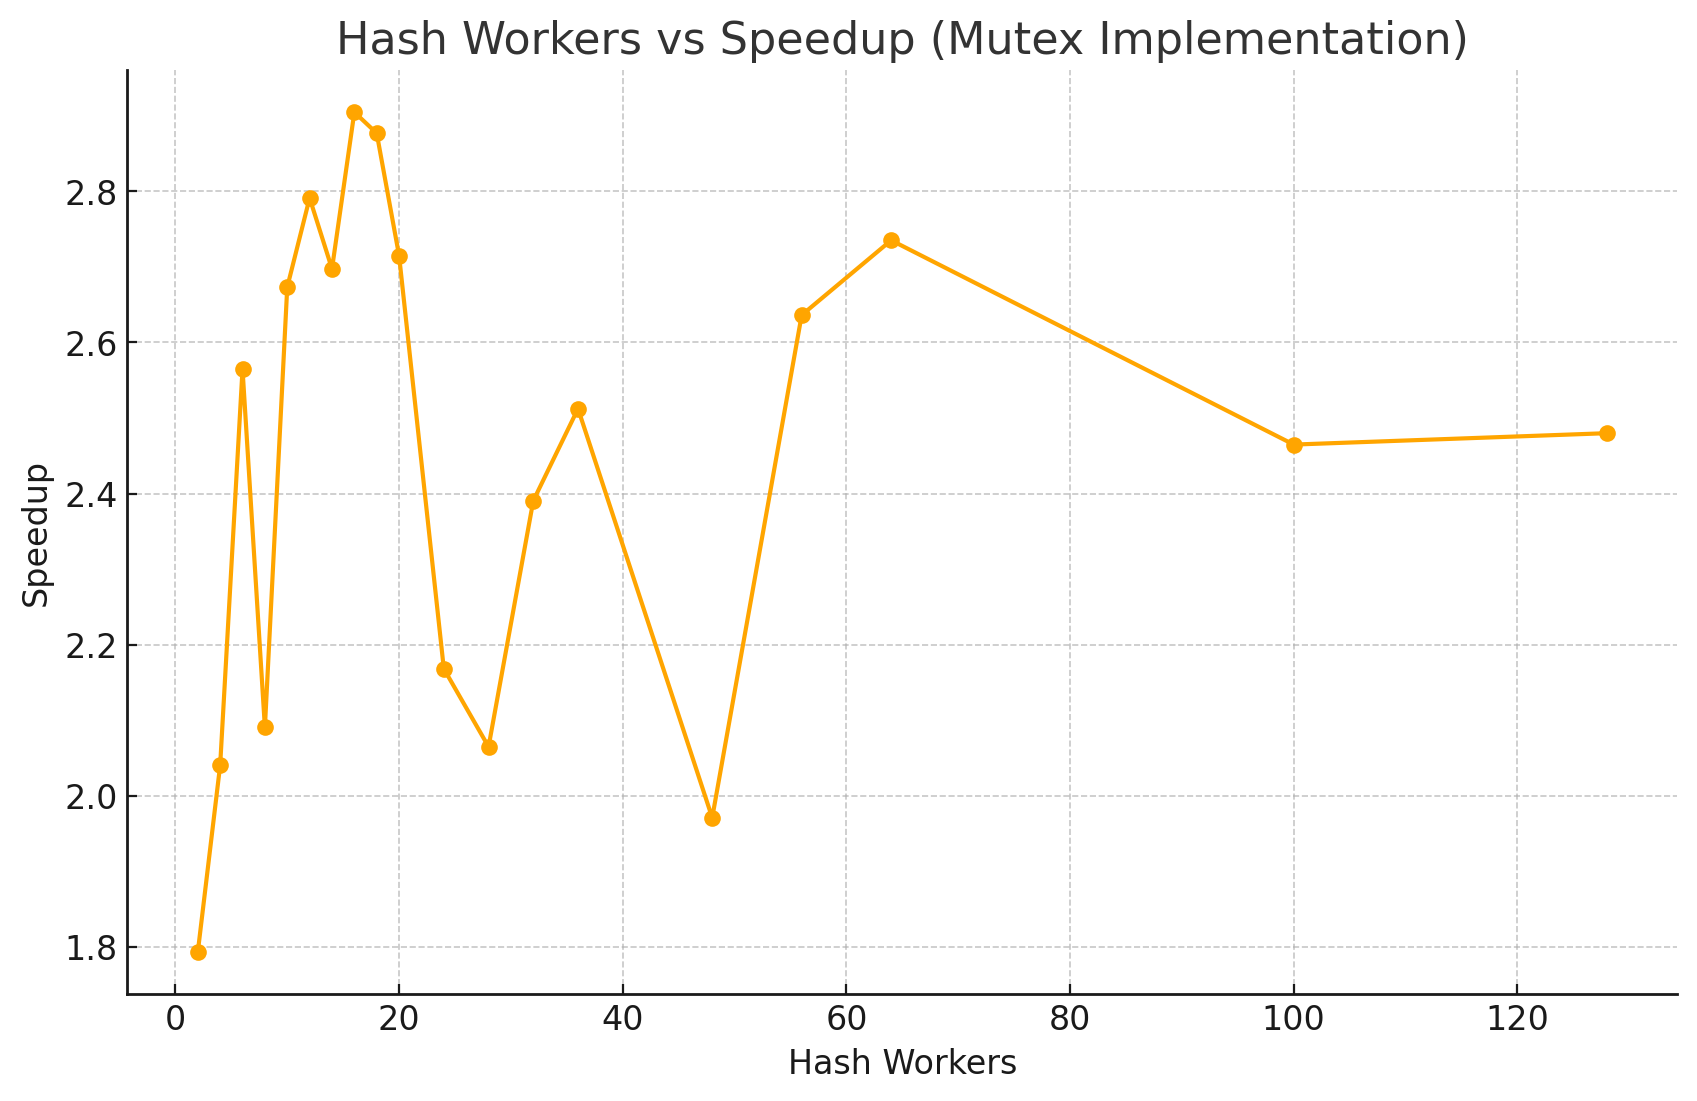
\includegraphics[width=0.7\textwidth]{mutexImplHash.png}
    \caption{Hashworkers vs SpeedUp for coarse.txt using mutex for coarse.txt}
    \label{fig:Hashworkers vs SpeedUp}
\end{figure}


\begin{figure}[ht]
    \centering
    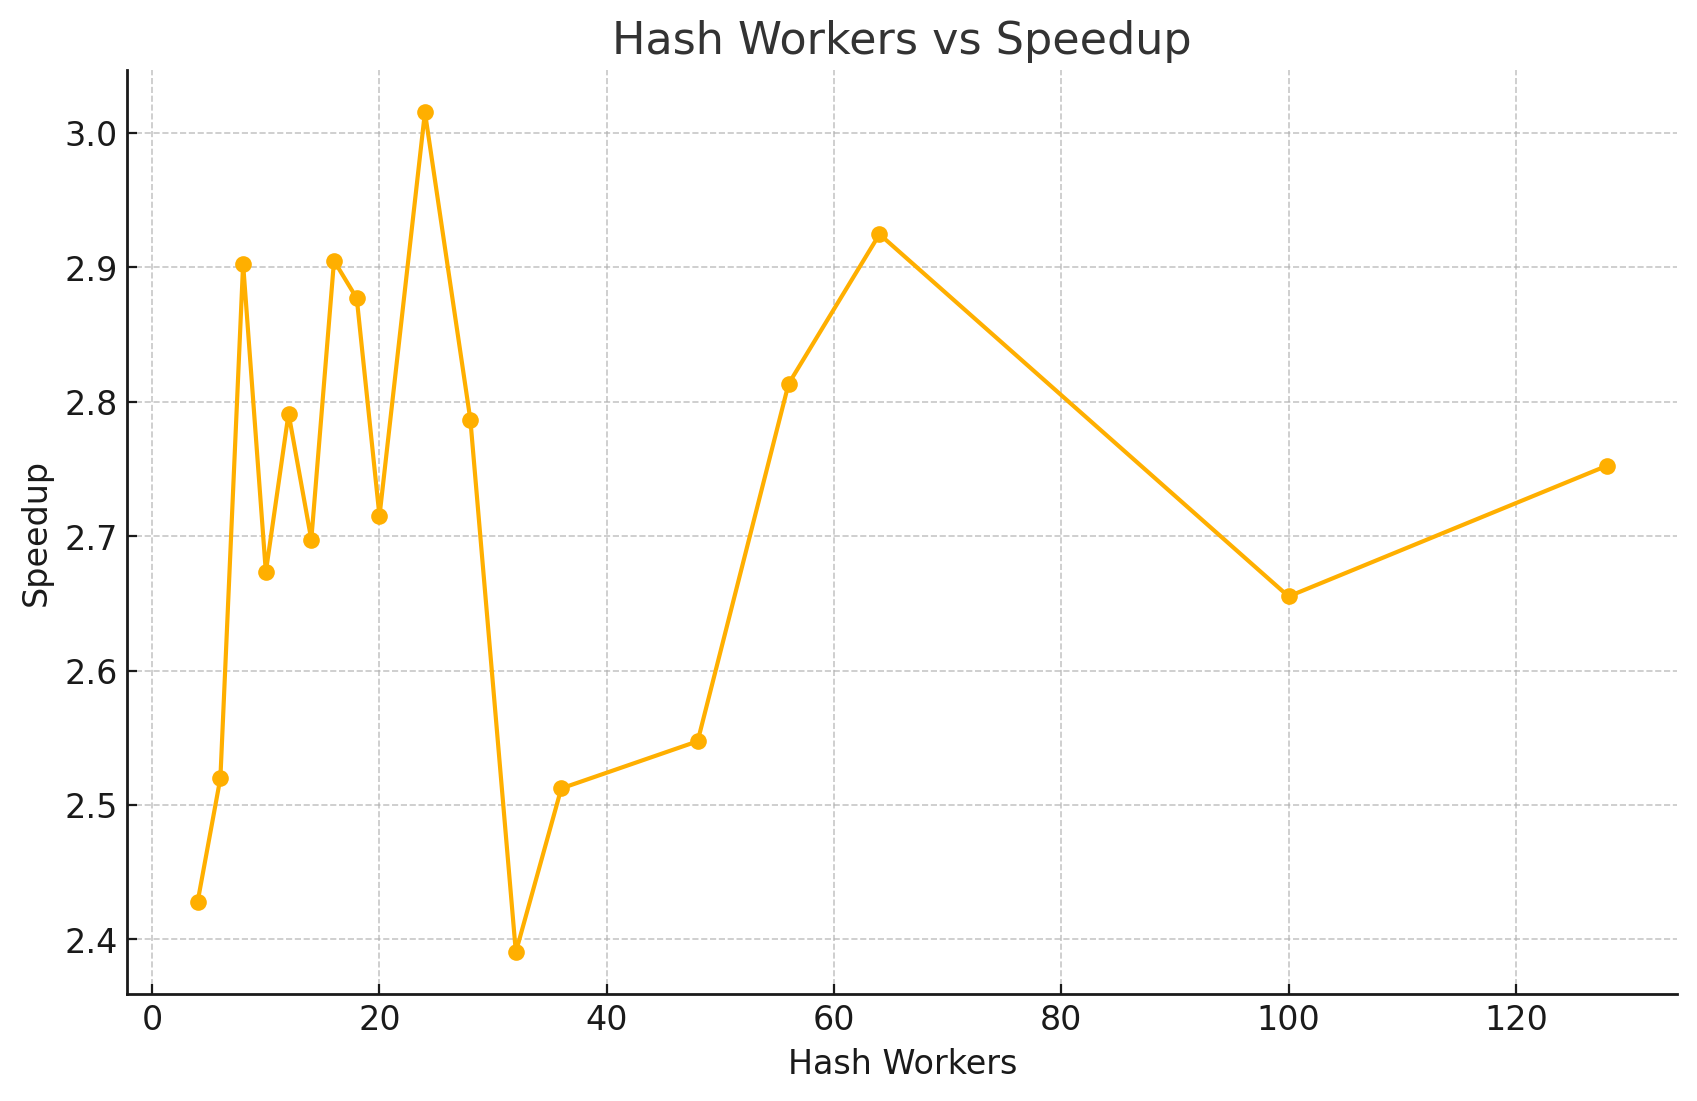
\includegraphics[width=0.7\textwidth]{semaphoreImplHash.png}
    \caption{Hashworkers vs SpeedUp  using semaphore for coarse.txt}
    \label{fig:Hashworkers vs SpeedUp}
\end{figure}



\begin{figure}[ht]
    \centering
    \includegraphics[width=0.7\textwidth]{hashworkerFine.png}
    \caption{Hashworkers vs SpeedUp  using channel for fine.txt}
    \label{fig:Hashworkers vs SpeedUp}
\end{figure}

\begin{figure}[ht]
    \centering
    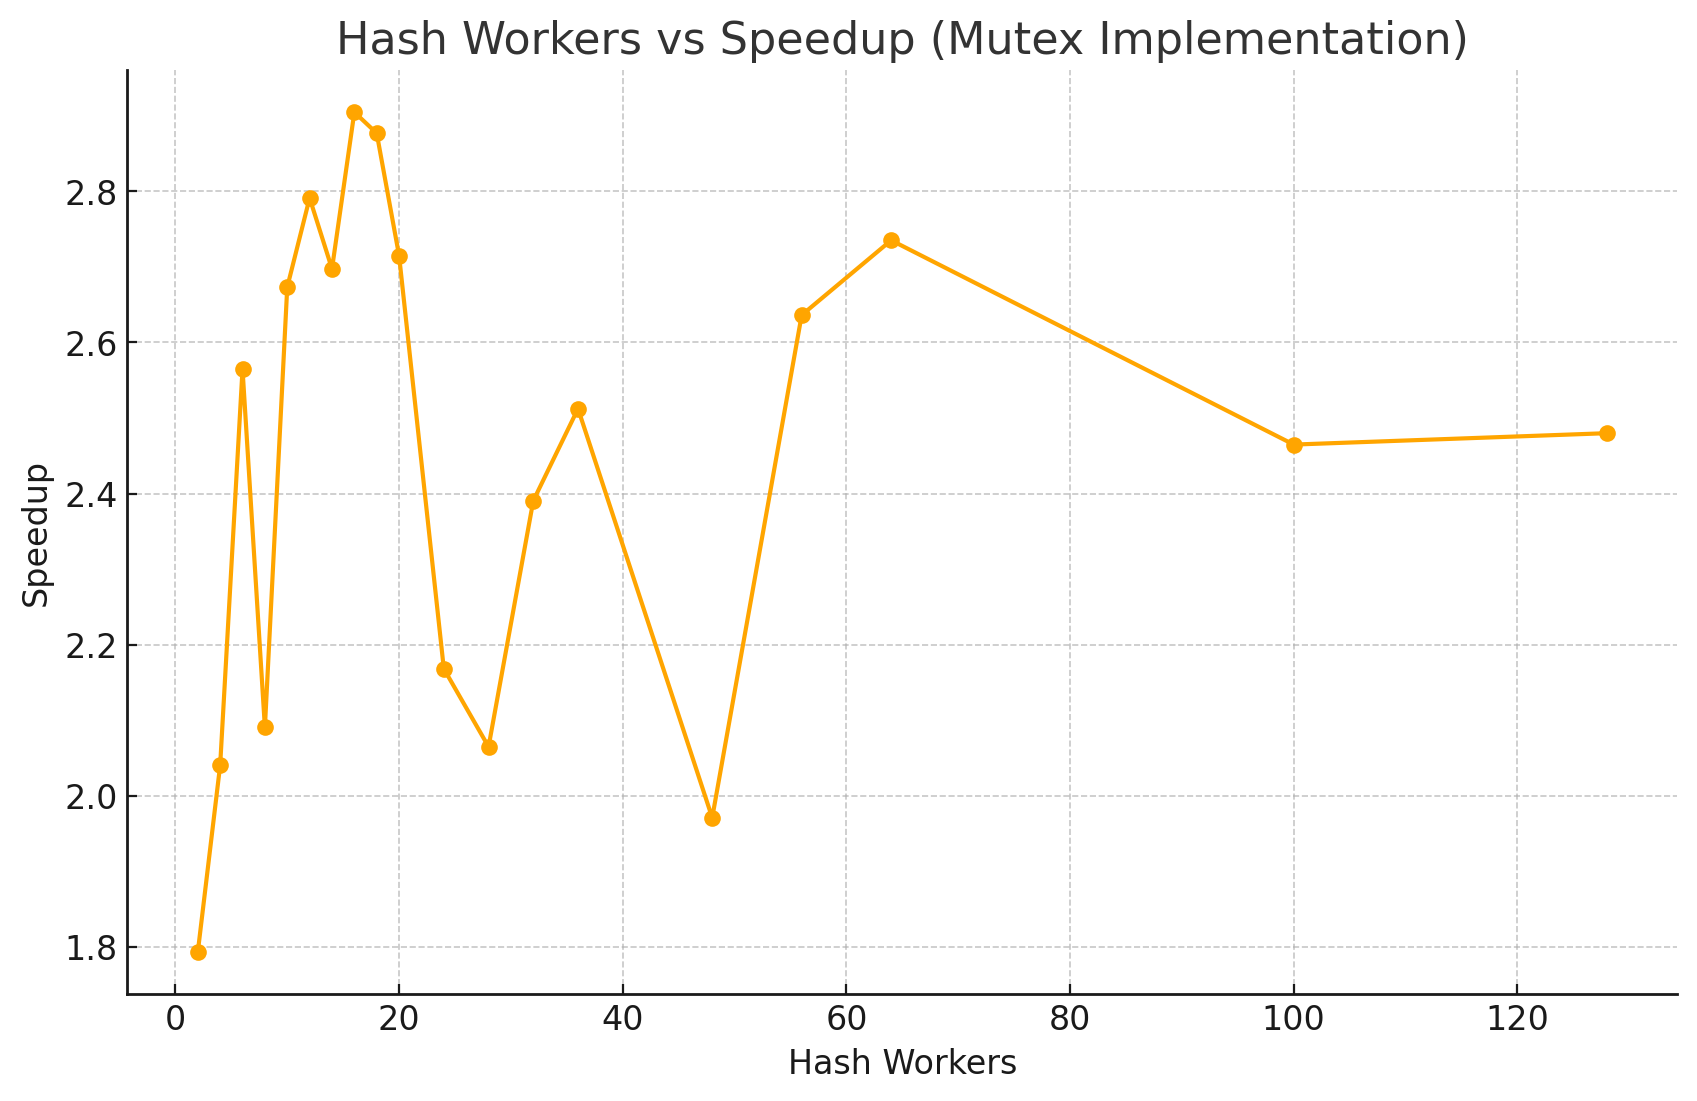
\includegraphics[width=0.7\textwidth]{hashworkerMutexFine.png}
    \caption{Hashworkers vs SpeedUp  using mutex for fine.txt}
    \label{fig:Hashworkers vs SpeedUp}
\end{figure}


\begin{figure}[ht]
    \centering
    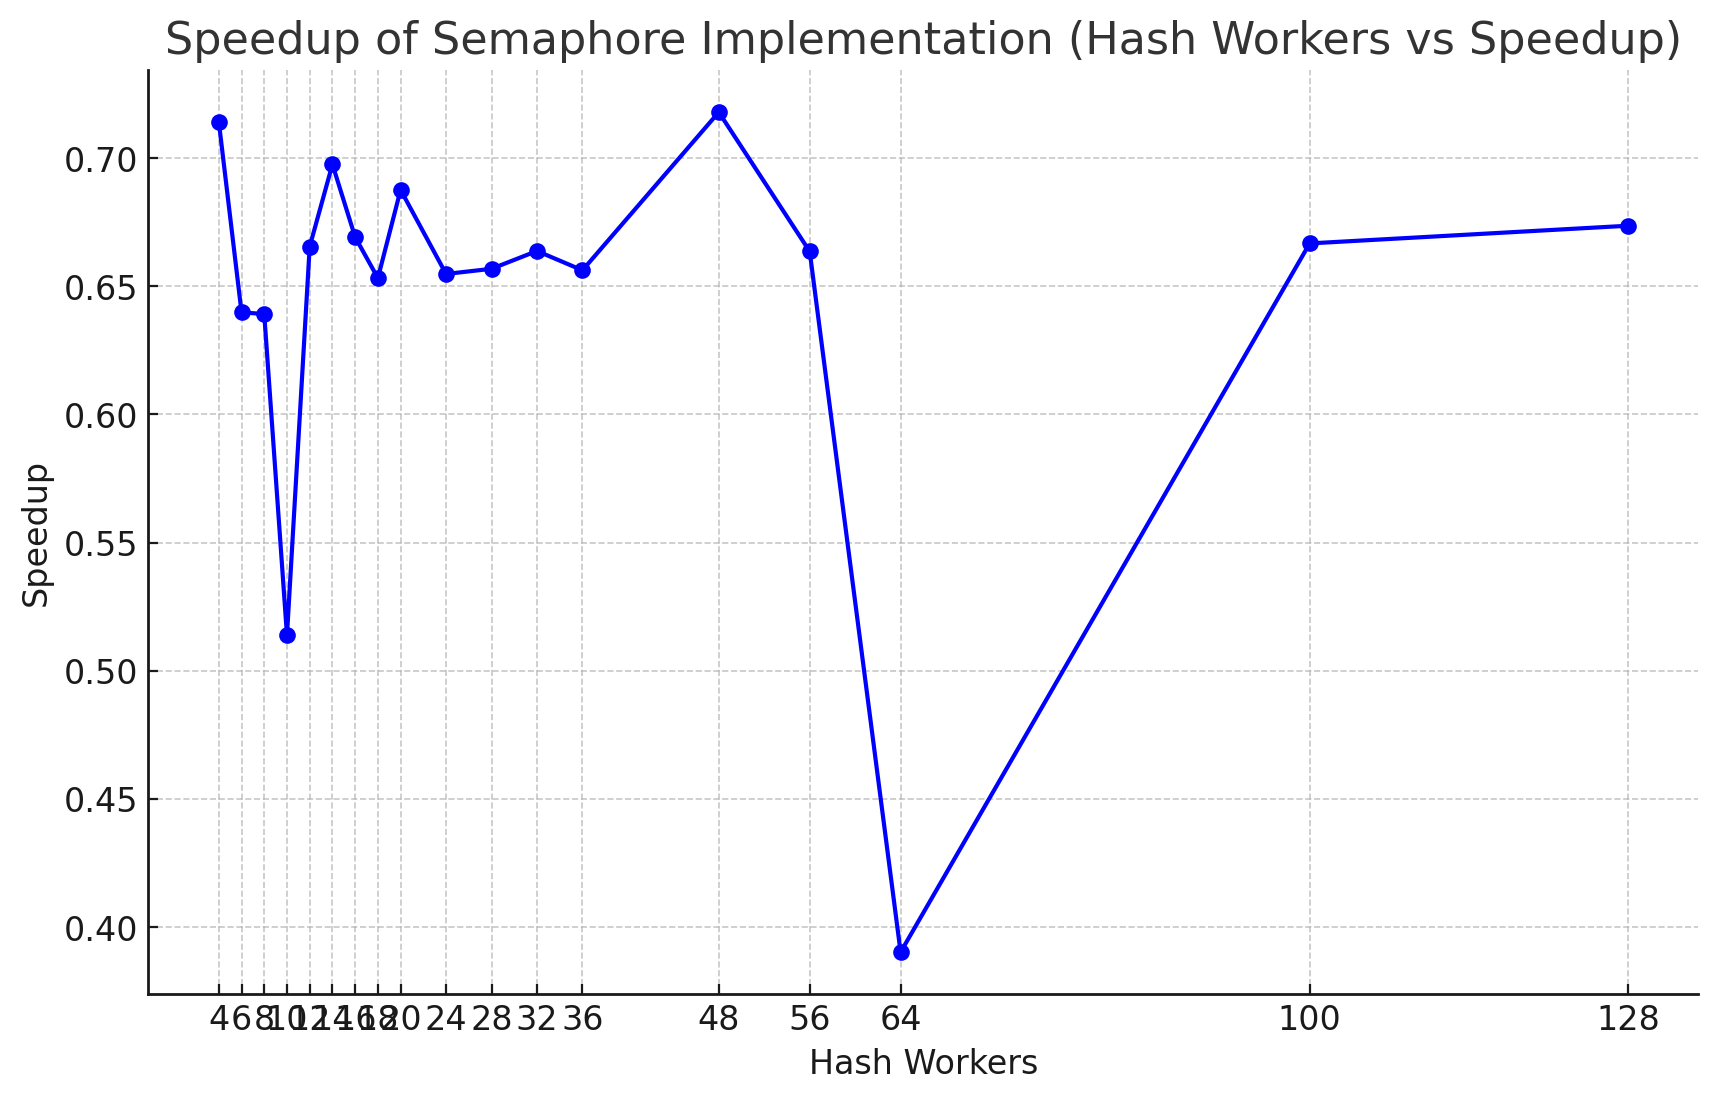
\includegraphics[width=0.7\textwidth]{hashworkerSemaphoreFine.png}
    \caption{Hashworkers vs SpeedUp  using semaphore for fine.txt}
    \label{fig:Hashworkers vs SpeedUp}
\end{figure}

\clearpage

\subsubsection{Tree Comparison Time}
% Comparison of tree comparison time for different `-comp-workers` configurations.

\begin{table}[h]
\centering
\begin{tabular}{|c|c|}
\hline
\textbf{comp-workers} & \textbf{compareTreeTime} \\ \hline
1   & 0.00057900 \\ \hline
2   & 0.00033346 \\ \hline
4   & 0.00026146 \\ \hline
6   & 0.00024288 \\ \hline
7   & 0.00042671 \\ \hline
8   & 0.00278529 \\ \hline
9   & 0.00022721 \\ \hline
10  & 0.00054133 \\ \hline
12  & 0.00021196 \\ \hline
14  & 0.00043604 \\ \hline
16  & 0.00024308 \\ \hline
18  & 0.00136396 \\ \hline
20  & 0.00059437 \\ \hline
24  & 0.00138379 \\ \hline
28  & 0.00024963 \\ \hline
32  & 0.00022996 \\ \hline
36  & 0.00077021 \\ \hline
48  & 0.00226400 \\ \hline
56  & 0.00025721 \\ \hline
64  & 0.00027312 \\ \hline
100 & 0.00035492 \\ \hline
128 & 0.00075346 \\ \hline
\end{tabular}
\caption{Comparison of Tree Times by Number of Workers for coarse.txt}
\label{table:comp_tree_times}
\end{table}




\begin{table}[h]
\centering
\begin{tabular}{|c|c|}
\hline
\textbf{comp-workers} & \textbf{compareTreeTime} \\ \hline
1  & 0.04143842 \\ \hline
2  & 0.05584687 \\ \hline
4  & 0.04198763 \\ \hline
6  & 0.03719104 \\ \hline
7  & 0.03862433 \\ \hline
8  & 0.03703254 \\ \hline
9  & 0.03675567 \\ \hline
10 & 0.03453496 \\ \hline
12 & 0.04155637 \\ \hline
14 & 0.03429696 \\ \hline
16 & 0.04181454 \\ \hline
18 & 0.03734808 \\ \hline
20 & 0.04253371 \\ \hline
24 & 0.03834558 \\ \hline
28 & 0.03861767 \\ \hline
32 & 0.04101271 \\ \hline
36 & 0.04212392 \\ \hline
48 & 0.05031371 \\ \hline
56 & 0.04995446 \\ \hline
64 & 0.05237017 \\ \hline
100& 0.06949183 \\ \hline
128& 0.07367017 \\ \hline
\end{tabular}
\caption{Comparison Workers and Tree Comparison Time for fine.txt}
\label{table:workers_time}
\end{table}

\clearpage

\begin{figure}[ht]
    \centering
    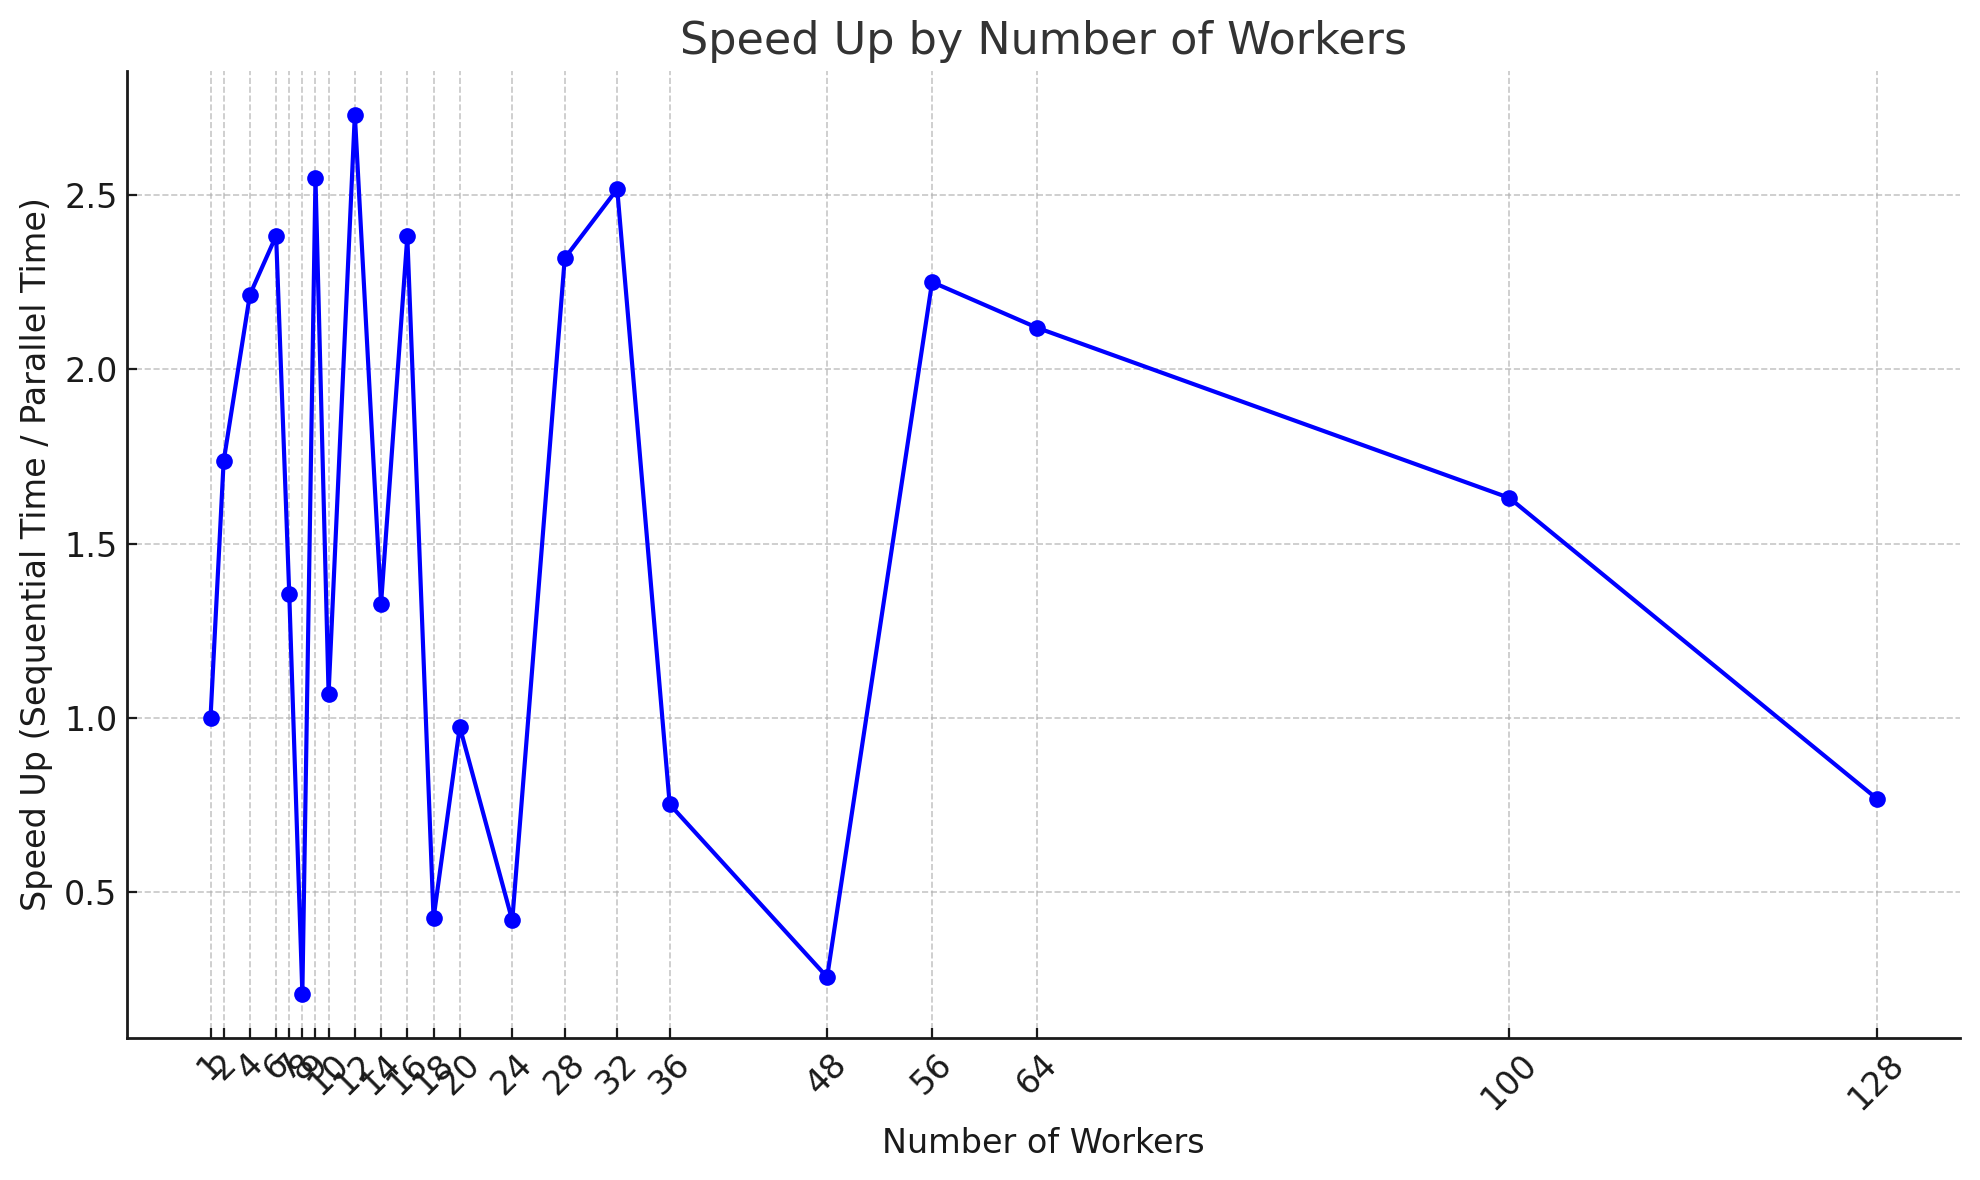
\includegraphics[width=0.7\textwidth]{compworkerSpeedUpcoarse.png}
    \caption{comp workers vs SpeedUp  for coarse.txt}
    \label{fig:Hashworkers vs SpeedUp}
\end{figure}


\begin{figure}[ht]
    \centering
    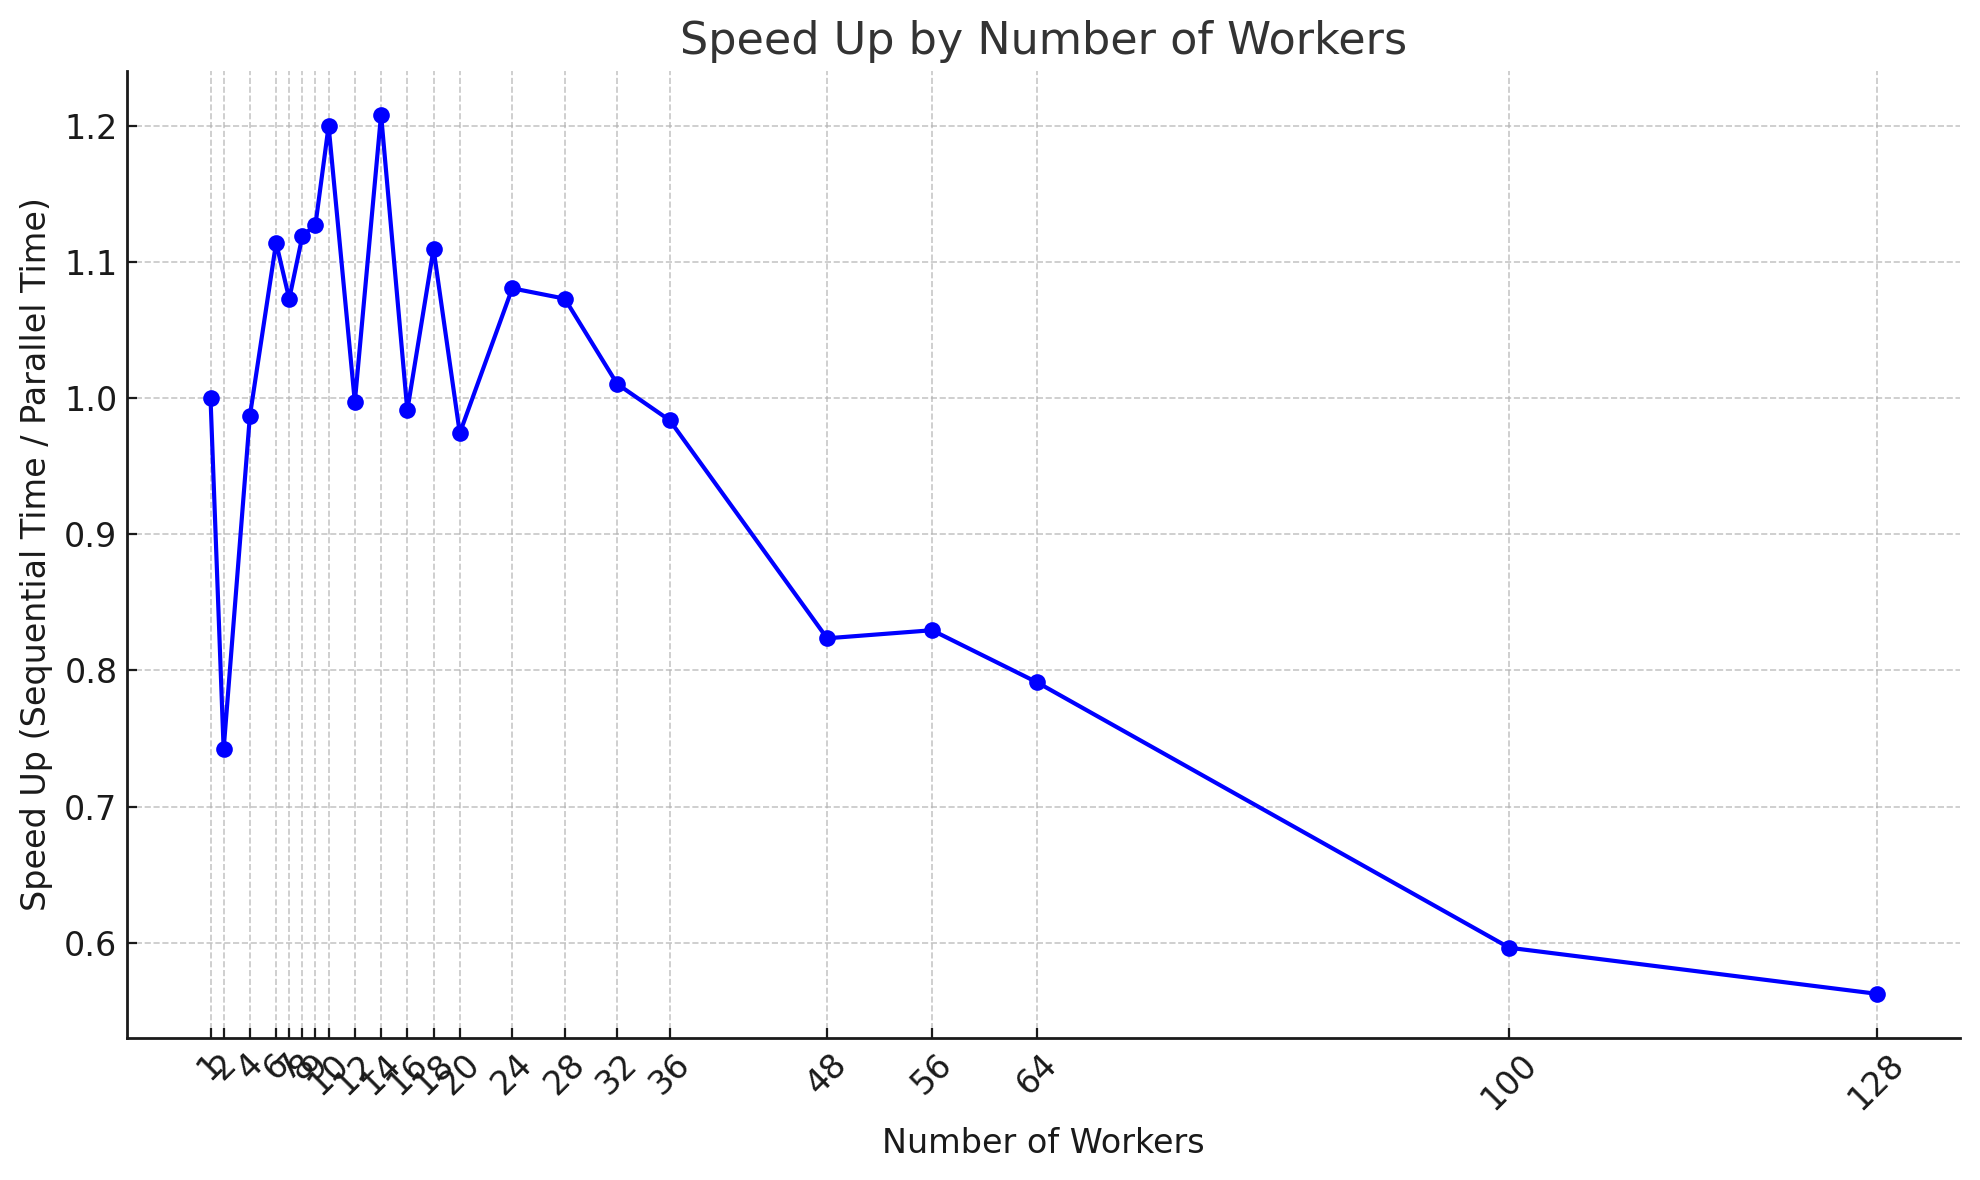
\includegraphics[width=0.7\textwidth]{compworkerSpeedUpfine.png}
    \caption{comp workers vs SpeedUp for fine.txt}
    \label{fig:Hashworkers vs SpeedUp}
\end{figure}



\subsection{Correctness Verification}
The output is same with expected output provided by one of the student.
% Results of output validation and correctness checks against reference data.
\begin{figure}[ht]
    \centering
    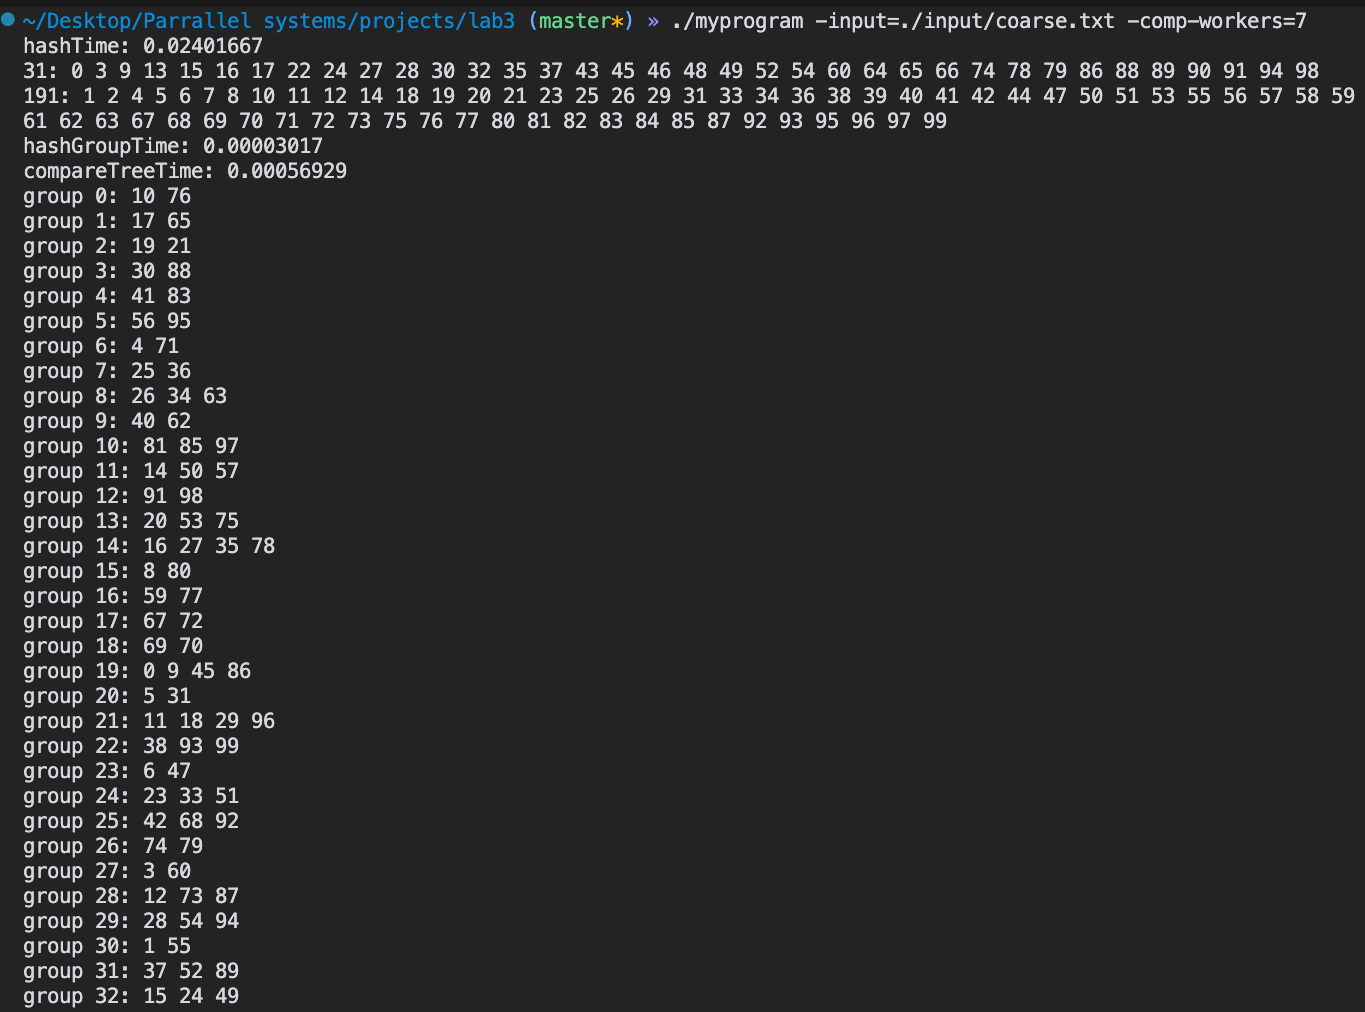
\includegraphics[width=0.8\textwidth]{correctness.png}
    \caption{correctness validation}
    \label{fig:Hashworkers vs SpeedUp}
\end{figure}




\clearpage


\section{Discussion}
% Discussion of concurrency trade-offs, synchronization overhead, and observed performance trends. Analysis of where parallelism was most effective and limitations encountered.

\subsection{Channel Implementation}
\begin{itemize}
    \item \textbf{Concurrent Processing:} As we can see from the graphs, Channel-based implementation excels with larger input size,  the workload is large enough to benefit from multiple workers processing in parallel, significantly reducing the total computation time, and result is more consistent.
    \item \textbf{Reduced Contention:} This approach minimizes direct contention for shared resources by using channels for communication, which can lead to improved throughput on larger datasets.
    \item \textbf{Overhead and Blocking:} The overhead associated with managing channels and potential blocking on channel operations can become a bottleneck, especially with smaller or unevenly distributed workloads.
\end{itemize}

\subsection{Mutex Implementation}
\begin{itemize}
    \item \textbf{Direct Map Access:} Mutex implementation allows workers to directly update the shared map, potentially reducing the complexity of data handling compared to channel-based approaches. 
     \item \textbf{Contention Issues:} The use of a single mutex can lead to significant contention, especially with a high number of concurrent workers, which can negate the benefits of parallelism. That is why with higher number of workers, the speedup drops.
    \item \textbf{Scalability Concerns:} While simpler to implement, the scalability of this method is limited by the mutex's ability to handle high contention levels effectively. Which is why we can see from the graphs, speedup for mutex impl for coarse.txt and fine.txt does not differ too much.
\end{itemize}

\subsection{Semaphore Implementation}
\begin{itemize}
    \item \textbf{Fine-grained Locking:} By using semaphores or fine-grained locking strategies, this implementation can offer better performance scaling by reducing the contention seen in single-mutex setups.
    \item \textbf{Complexity and Overhead:} However, managing multiple locks or semaphores introduces additional complexity and synchronization overhead, which might not always translate to proportionate performance gains. Which is why we can see for larger input of semaphore speedup graph, there isn't much speedup comparing to sequential implementation. But for medium sized input file, we do observe some kind of speedup.
    \item \textbf{Optimal for Medium to Large Workloads:} Semaphore strategies are most effective for medium to large workloads where the overhead can be justified by significant performance improvements over simpler locking mechanisms.
\end{itemize}

\subsection{Comparison Workers and Speedup Analysis}
We do not observe liner speed up, adding more comp workers suffers from some overheads introduced in task scheduling, worker synchronization. While it does speedup better for coarse.txt with medium sized input, it does not scale well for the larger size input. \\\\
Tasks (tree comparisons) are distributed to compWorkers via channels. This involves dynamically allocating pairs of trees to be compared and managing these tasks through channels. Each time a task is sent through a channel, there's an overhead associated with context switching and managing these communications. As the number of workers increases, the overhead associated with scheduling and distributing these tasks also grows.\\\\
Depending on how the tree comparisons are batched and distributed, some workers might end up with more work than others. This imbalance can cause some workers to be idle while others are still processing, reducing overall efficiency.



\subsubsection{Impact of Number of Workers}
\begin{itemize}
    \item \textbf{Few Workers:} With too few workers, the potential for parallel processing is not fully realized, often leading to underutilization of available processing resources.
    \item \textbf{Many Workers:} Conversely, too many workers can lead to excessive context switching, increased contention for shared resources, and overall inefficiency, particularly when the number of workers exceeds the number of processing cores.
    \item \textbf{Optimal Number of Workers:} The optimal number of workers typically lies between these two extremes and is dependent on the specific characteristics of the hardware and the nature of the tasks being processed.
\end{itemize}

\subsubsection{Recommendations for Optimization}
\begin{itemize}
    \item \textbf{Dynamic Worker Allocation:} Implementing a dynamic worker allocation strategy that adjusts the number of workers based on the workload can help in achieving near-optimal performance across different scenarios.
    \item \textbf{Workload Balancing:} Efforts should be made to ensure that the workload is evenly distributed among the available workers to avoid bottlenecks and idle resources.
    \item \textbf{Hardware Considerations:} Understanding the underlying hardware capabilities, such as the number of cores and the memory hierarchy, can guide the configuration of the parallel execution environment to better align with the system’s strengths.
\end{itemize}

This analysis underscores the importance of carefully selecting the number of comparison workers to maximize the efficiency of parallel tree comparisons. The insights derived from speedup metrics assist in fine-tuning the concurrency model to better harness the computational power available, ensuring that the parallel algorithm performs optimally under varying operational conditions.


\subsection{General Observations}
\begin{itemize}
    \item \textbf{Performance with Larger Inputs:}
    \begin{itemize}
        \item parallel implementations tend to perform better with larger input sizes where the benefits of concurrent execution outweigh the overhead of managing parallel processes, even thought this observation may not hold true for all the implementations.
    \end{itemize}
    
    \item \textbf{Performance with Smaller Inputs:}
    \begin{itemize}
        \item Challenges such as setup cost, task granularity, and sensitivity to system conditions often result in less consistent performance with smaller datasets.
    \end{itemize}
    
    \item \textbf{Optimization Strategies:}
    \begin{itemize}
        \item Dynamic adjustment of the concurrency level and employing hybrid strategies that switch between sequential and parallel processing based on the input size could optimize performance across varying workloads.
    \end{itemize}
\end{itemize}


\section{Conclusion and Improvement Ideas}
% Summary of findings, key takeaways on parallel BST comparison, and potential improvements.

The analysis of BST comparison reveals significant insights into the behavior of different concurrency models under varying workloads. While the channel-based implementation showcases its strength in environments with larger datasets by efficiently minimizing contention and maximizing throughput, it struggles with overheads in smaller workloads. Conversely, mutex and semaphore implementations highlight trade-offs between simplicity and scalability, with mutexes facing bottlenecks in high contention scenarios and semaphores introducing complexity that may not always yield proportional benefits. The findings underscore the necessity of a balanced approach in worker allocation and task distribution to harness full computational capabilities. Optimizing the number of workers and refining synchronization mechanisms based on empirical data and hardware capabilities can significantly enhance the performance and scalability of the BST comparison application across diverse operational conditions.

\section*{References}


\subsection*{Technical Sources:}

\begin{itemize}

    \item \href{https://go.dev/doc/}{GoLang document}
    \item \href{https://go101.org/article/concurrent-synchronization-more.html}{Concurrency Synchronization Techniques Provided in the sync Standard Package}
    \item \href{https://medium.com/@deckarep/gos-extended-concurrency-semaphores-part-1-5eeabfa351ce}{gos-extended-concurrency-semaphores}
    \item \href{https://www.codingexplorations.com/blog/understanding-and-implementing-the-semaphore-pattern-in-go}{understanding-and-implementing-the-semaphore-pattern-in-go}
         \end{itemize}

\end{document}


